\chapter{Time Reversal}\label{chapter:TimeReversal}

Time-reversal methods involve mirroring the propagation of waves in time, aiming to converge the resulting wave back to its source.~\parencite{Fink2017} mentions two ways to achieve time-reversal.
The first method involves \ac{TRM}s, which rely on Cauchy boundary conditions. If the wavefield and its normal derivative are known at the entire surface $S$ surrounding the volume
$V$ at all times $t$, the wavefield inside the entire volume can be computed. In this approach, the outgoing wave is initially 
recorded on $S$, then time-reversed and finally emitted from $S$. \\

Alternatively, time-reversal can be achieved with manipulation of the initial conditions. In this case, the wavefield and its normal derivative
are known inside the entire volume but only for a specific time. 
~\parencite{Weinert2016} describes Loschmidt's demon as something hypothetical which reverses the momentum/velocity of each particle instantaneously such that the state of the system is reversed 
from a fibrillated state to a less fibrillated, smoother state.
By doing something which mimicks Loschmidt's demons ~\parencite{Weinert2016}, ~\parencite{Fink2017} which act simultaneously on the entire space, the velocity of each particle can be instantaneously reversed, resulting in a time-reversed wave. This approach is known as the \ac{ITM}.\\

This thesis primarily focuses on the \ac{ITM} approach for seismic waves. In this method, a time-reversed wave is generated through a sudden modification of the wave propagation
properties of the medium~\parencite{Bacot2016}. Section \ref{section:ITMTheory} delves into the theoretical foundation behind the \ac{ITM}, providing a comprehensive
understanding of its principles. In the latter part of the chapter, we present the implementation of \ac{ITM} within the numerical simulation software SeisSol. The
description of the implementation is kept as general as possible, allowing for a broad grasp of the method's application and utility.

\section{Theory of Instantaneous Time Mirrors}\label{section:ITMTheory}

Time-reversal methods for waves are based on the time-reversal invariance of wave equations. They rely on the fact that any wave-field can be completely determined within
a volume by knowing the field(and its normal derivative) on any enclosing surface~\parencite{Bacot2016}. We write the elastic wave equation in its second order vector form
~\parencite[Cha. 2]{aki2002quantitative} as
\begin{equation}
    \rho \ddot{\mathbf{U}} \left( \mathbf{x}, t\right) - \left( \lambda + 2 \mu \right) \nabla \left(\nabla \cdot \mathbf{U}\left(\mathbf{x}. t\right)\right) 
    + \mu \nabla \times \left(\nabla \times \mathbf{U}\left(\mathbf{x},t\right)\right) = \mathbf{S}\left(\mathbf{x},t\right),
\end{equation}

with the source function $\mathbf{S}\left(\mathbf{x},t\right)$ contains only second order time derivatives. This implies that if $\hat{\mathbf{U}}\left(\mathbf{x},t\right)$
is a solution, then $\hat{\mathbf{U}}\left(\mathbf{x}, -t\right)$ is also a solution, if $\mathbf{S}$ is symmetric in time such that 
$\mathbf{S}\left(\mathbf{x}, t\right) = \mathbf{S}\left(\mathbf{x}, -t\right)$. \\

The \ac{ITM} approach is closely connected to the Cauchy theorem, which states that the wave field evolution can be deduced from the knowledge of thie wave field
and its derivative at one single time, i.e., the initial conditions. By inducing a sudden modification of the wave propagation properties(such as impedance) in the
medium, a time-reversed wave is generated. This modification, referred to as the \ac{ITM}, does not require the use of antennas or the entire wave field's memory~\parencite{Bacot2016}.
~\parencite{Bacot2016} demonstrated this for water waves with physical and numerical experiments resulting in successful refocusing of the generated waves into their
sources' shapes. This was achieved by introducing a temporal slab in the wave velocities like in figure \ref{fig:deltavelocity}

\begin{figure}
    \centering
    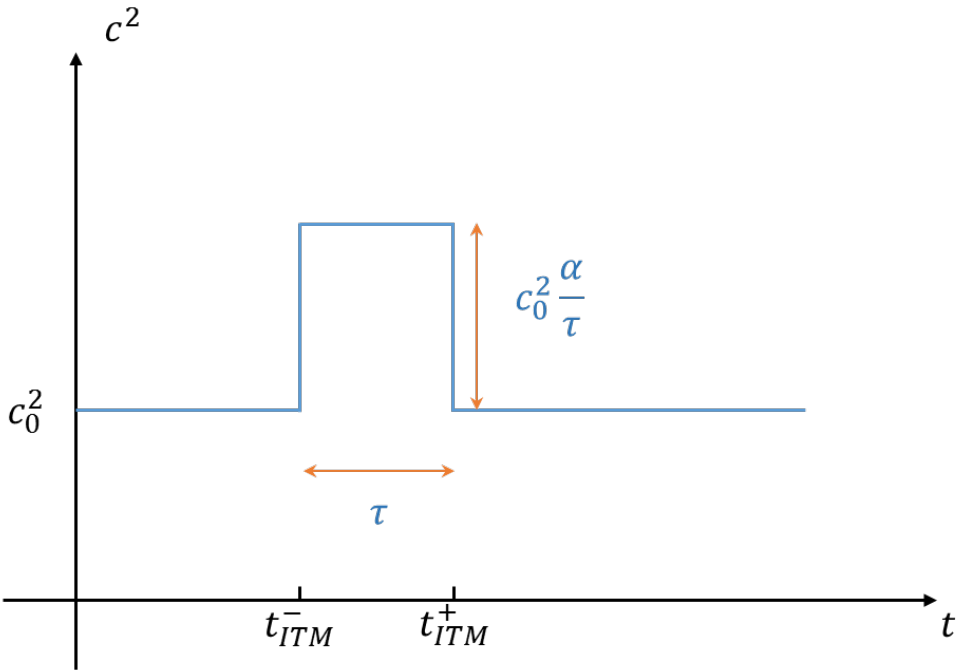
\includegraphics[width=0.6\linewidth]{figures/delta_speed.png}
    \caption{Rectangular profile for the wave velocity. Properties of the wave are changed during the duration of \ac{ITM}. (Figure taken from Figure 1 in ~\parencite[Supplementary Material]{Bacot2016})}
    \label{fig:deltavelocity}
\end{figure}

In the context of elastic waves, as we have seen in equations \ref{eq:setofequations} and \ref{eq:wavevelocities}, there are two propagating waves, i.e., P- and S- waves. 
~\parencite[Sec 9.6-Sec 9.8]{leveque_2002} shows that in case of spacial material interfaces, a discontinuity in the quantity called Impedance $Z = \rho v$
causes reflections across the material interface. ~\parencite[Eq. 1.66 and 1.180]{kaufman} show that impedances of P- and S- waves are defined analogously as
$Z_p = \rho v_p$ and $Z_s = \rho v_s$.